\documentclass[../../statistical_learning_notes.tex]{subfiles}
\begin{document}
%%%%%%%%%%%%%%%%%%%%%%%%%%%%%%%%%%%%%%%%%%%%%%%%%%%%%%%%%%%%%%%%%%%%%%%%%%%
\section{Sampling from Distributions}
\subsection{Rejection Sampling}
Consider a probability distribution $p(x)$ that we want to sample from, and suppose there is another distribution $q(x)$ such that $p(x) \leq Mq(x)$ where $M$ is a constant scalar. Assume that $q$ is a distribution from which we can easily sample. Then to sample from $p(x)$
\begin{enumerate}
    \item Sample a point $x_{0}$ from $q(x)$
    \item Sample a point $u$ from $Uniform(0,Mq(x_{0}))$
    \item Accept $x_{0}$ with probability $\frac{p(x_{0})}{Mq(x_{0})}$ if $u \leq p(x_{0})$
\end{enumerate}

The scheme works because any point we are accepting lies inside the curve $p(x)$. Also, on average, we will get $1$ accepted point for every $M$ samples because the total points generated cover the area under $q(x)$ while the accepted ones cover the area under $Mq(x)$. The total points accepted are simply the ratios of area under $p(x)$ and $M(q(x)$.\newline

The technique works equally well if we know the distribution only upto a normalization constant
\begin{gather*}
    \frac{\tilde{p}(x)}{Z} \leq Mq(x) \implies \tilde{p}(x) \leq M^{\prime}q(x), \; M^{\prime} = ZM
\end{gather*}

\begin{figure}[h]
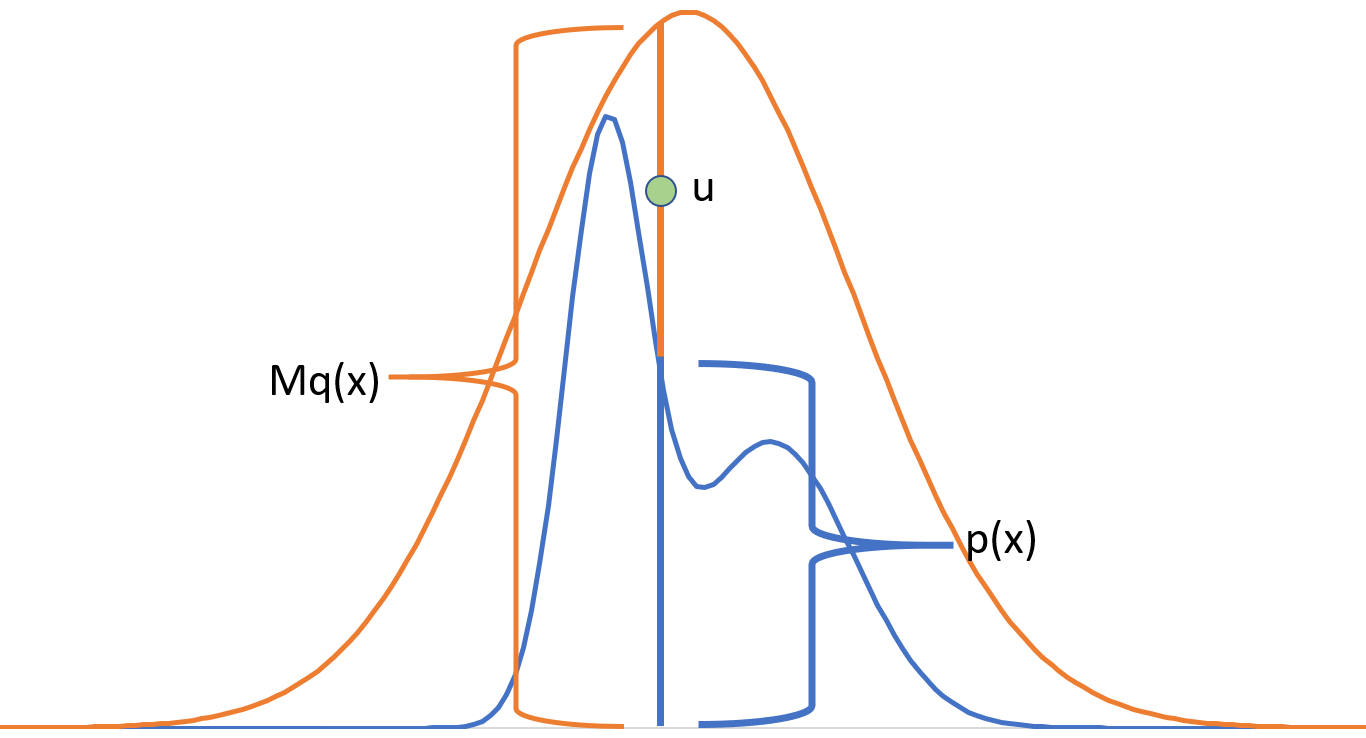
\includegraphics[scale=0.3]{sampling_1}
\centering
\caption{Rejection Sampling: $u$ is selected with probability $p(x)/Mq(x)$}
\label{fig:sampling_1} %\ref{fig:sampling_1}
\end{figure}


%%%%%%%%%%%%%%%%%%%%%%%%%%%%%%%%%%%%%%%%%%%%%%%%%%%%%%%%%%%%%%%%%%%%%%%%%%%
\subsection{Gibbs Sampling}
Gibbs Sampling is a markov chain based sampling method which samples from a multivaraiate distribution one component at a time. Specifically, any component is sampled using a conditional distribution on all the remaining components, where we use the latest available values for those components. Suppose we are sampling from a $d$ dimensional distribution $p(x)$
\begin{enumerate}
    \item Initialize ($x_{1}^{(0)},\ldots x_{d}^{(0)}$) as random values or zeros
    \item For $k = 0,1,2,\ldots$
    \begin{align*}
        x_{1}^{(k+1)} &\sim p(x_{1}|x_{2}^{(k)},\ldots x_{d}^{(k)})\\
        x_{2}^{(k+1)} &\sim p(x_{2}|x_{1}^{(k+1)},x_{3}^{(k)},\ldots x_{d}^{(k)})\\
        x_{3}^{(k+1)} &\sim p(x_{3}|x_{1}^{(k+1)},x_{2}^{(k+1)},x_{4}^{(k)},\ldots x_{d}^{(k)})\\
        \vdots\\
        x_{d}^{(k+1)} &\sim p(x_{d}|x_{1}^{(k+1)},x_{2}^{(k+1)},\ldots x_{d-1}^{(k+1)})\\
    \end{align*}
\end{enumerate}

Each of the samplings steps involve a single variable. This sampling is easy if we know a good sampling procedure for the same already, or something generic like rejection sampling can be used.\newline

This iterative procedure works because
\begin{gather*}
    p(x_{1}^{(k+1)},\ldots,x_{d}^{(k+1)}) = \sum_{x_{1}^{(k)},\ldots,x_{d}^{(k)}} Q(x_{1}^{(k)},\ldots,x_{d}^{(k)} \rightarrow x_{1}^{(k+1)},\ldots,x_{d}^{(k+1)}) p(x_{1}^{(k)},\ldots,x_{d}^{(k)})\\
    Q = p(x_{1}^{(k+1)}|x_{2}^{(k)},\ldots x_{d}^{(k)})p(x_{2}^{(k+1)}|x_{1}^{(k+1)},x_{3}^{(k)},\ldots x_{d}^{(k)}) \ldots p(x_{d}^{(k+1)}|x_{1}^{(k+1)},x_{2}^{(k+1)},\ldots x_{d-1}^{(k+1)})
\end{gather*}
which can be solved by breaking the sum over the different components and marginalizing the sum one component at a time. $Q$ is nothing but the transition probability of the markov chain.\newline

Since the procedure uses a markov chain, we disregard some of the initial points as the chain may not have converged till then. This is called the burn-in period (say 1000 samples). Further, it is sually the case that successive samples have high degree of correlation between. To avoid this, after the burn-in period has passed, we only keep every $k^{th}$ (say 100) observation in the final set of samples. The procedure works even if the distribution is known only upto a normalization constant.


%%%%%%%%%%%%%%%%%%%%%%%%%%%%%%%%%%%%%%%%%%%%%%%%%%%%%%%%%%%%%%%%%%%%%%%%%%%
\subsection{Metropolis Hastings}
Metropolis Hastings uses the concept of rejection sampling and markov chains to develop and efficient sampling procedure. Unlike the fixed transition probabilities in Gibbs sampling, we have the freedom to choose the appropriate transition function here, to produce less correlated samples.

Consider a markov chain $Q$ that will define transition probabilities and sampling procedure, a critic $A$ that will tell us to accept or reject a sampled point and $T$ as the final markov chain. Then,
\begin{align*}
    T(\bm{x}\rightarrow \bm{x}^{\prime}) = Q(\bm{x} \rightarrow \bm{x}^{\prime})A(\bm{x} \rightarrow \bm{x}^{\prime})
\end{align*}
which we want to be stationary.
\begin{align*}
    \text{Assume} \quad \pi(\bm{x})T(\bm{x} \rightarrow \bm{x}^{\prime}) &= \pi(\bm{x}^{\prime})T(\bm{x}^{\prime} \rightarrow \bm{x})\\
    \implies \sum_{\bm{x}} \pi(\bm{x})T(\bm{x} \rightarrow \bm{x}^{\prime}) &= \sum_{\bm{x}} \pi(\bm{x}^{\prime})T(\bm{x}^{\prime} \rightarrow \bm{x}) = \pi(\bm{x}^{\prime})
\end{align*}
which is the stationarity condition for a markov chain and $\pi$ denote the long term stationary probabilities. These are indeed the probability distribution $P$ we are trying to approximate. To check stationarity, we only need to work with the first equation and choose $A$ accordingly
\begin{alignat*}{2}
    \pi(\bm{x})Q(\bm{x} \rightarrow \bm{x}^{\prime})A(\bm{x} \rightarrow \bm{x}^{\prime}) &= \pi(\bm{x}^{\prime})Q(\bm{x}^{\prime} \rightarrow \bm{x})A(\bm{x}^{\prime} \rightarrow \bm{x})\\
    \frac{A(\bm{x} \rightarrow \bm{x}^{\prime})}{A(\bm{x}^{\prime} \rightarrow \bm{x})} &= \frac{\pi(\bm{x}^{\prime})Q(\bm{x}^{\prime} \rightarrow \bm{x})}{\pi(\bm{x})Q(\bm{x} \rightarrow \bm{x}^{\prime})} = \rho\\
    A(\bm{x} \rightarrow \bm{x}^{\prime}), A(\bm{x}^{\prime} \rightarrow \bm{x}) &= \begin{cases} \rho, 1 &\mbox{if $\rho < 1$}\\
    1, 1/\rho &\mbox{otherwise} \end{cases}\\
    \implies A(\bm{x} \rightarrow \bm{x}^{\prime}) &= \min \bigg(1, \frac{\pi(\bm{x}^{\prime})Q(\bm{x}^{\prime} \rightarrow \bm{x})}{\pi(\bm{x})Q(\bm{x} \rightarrow \bm{x}^{\prime})}\bigg)
\end{alignat*}
when $\rho < 1$, we keep $A(\bm{x} \rightarrow \bm{x}^{\prime}) = \rho$ so as to maximize the acceptance probability (other combinations like fractions of $\rho$ will also work, but will have lower acceptance probability). $A$ is also a probability distribution and $\in [0,1]$.\newline

The Metropolis Hastings Algorithm becomes
\begin{enumerate}
    \item Initialize $\bm{x}^{(k)}$ randomly
    \item For $k = 1, 2, \ldots$
    \begin{enumerate}
        \item Sample $\bm{x}^{\prime} \sim Q(\bm{x}^{(k)} \rightarrow \bm{x}^{\prime})$
        \item Calculate acceptance probability as
        \begin{align*}
            \rho = \min \bigg(1, \frac{P(\bm{x}^{\prime})Q(\bm{x}^{\prime} \rightarrow \bm{x})}{P(\bm{x})Q(\bm{x} \rightarrow \bm{x}^{\prime})} \bigg)
        \end{align*}
        \item With probability $\rho$, $\bm{x}^{(k+1)} = \bm{x}^{\prime}$ else $\bm{x}^{(k)}$
    \end{enumerate}
\end{enumerate}

A very naive choice of $x^{\prime} \sim Q(\bm{x} \rightarrow \bm{x}^{\prime}) = \mathcal{N}(\bm{x}, \bm{I})$. A few points about Metropolis Hastings algorithm
\begin{itemize}
    \item The algorithm is rejection sampling applied at markov chains
    \item There is a burn-in period and we will reject some of the initial samples (say 1000) to allow the chain to stabilize
    \item We have the choice over $Q$ which can be a family of distributions. Different choices of $Q$ will lead to different rates of convergence
    \item The method can be executed in parallel by running different chains on different machines
    \item Unnormalized distributions can also be sampled from since we have the ratio term in $A$
\end{itemize}
\end{document}